\documentclass[a4paper,oneside]{memoir}
\usepackage[utf8]{inputenc}
\usepackage{microtype}
\usepackage{graphicx}
\usepackage[linkbordercolor={0.8 0.8 1}]{hyperref} % muss letztes package sein
\title{EasyFlash Programmer's Guide}
\author{
Thomas 'skoe' Giesel
(skoe@directbox.com)
}

\begin{document}
\emergencystretch=0.15\hsize
\maketitle

\tableofcontents

\chapter{Introduction}

This manual gives you all information to start to develop software for the
EasyFlash cartridge in a low-level way.

\section{Additional Reading}

When you finished this Programmer's Guide, you may want to find out more about
high level mechanisms like the EasyFlash File System and related formats and
tools. You can find information about these in EasyFlash-EasyFS.pdf.

\chapter{Hardware Description}

\section{Flash Memory Configuration}

An EasyFlash cartridge consists of two flash memory chips, called ROML chip and ROMH chip. Each of them has a size of 512 KiB. Even though newer EasyFlash versions have only one physical chip, they can still be seen as these two logical chips.

As only 8 KiB of memory per chip can be mapped into the address space of the C64 at once, EasyFlash supports banking. Each chip has a size of 512 KiB, so there are 512 / 8 = 64 banks.

The mapping of the chips into the C64 memory is controlled by two lines of the Expansion Port: /GAME and /EXROM. Table \ref{tab:game-exrom} shows the possible memory configurations. Keep in mind that also the CPU register \$01 influences the memory configuration.

\begin{table}[!htbp]
    \centering
    \begin{tabularx}{\textwidth}{ccllX}
        \toprule
        /GAME & /EXROM & ROML & ROMH & Mode \\
        \midrule
        1 & 1 &     -               & -                 & Invisible Mode \\[3pt]
        1 & 0 &     8 KiB at \$8000 & -                 & 8K Mode  \\[3pt]
        0 & 0 &     8 KiB at \$8000 & 8 KiB at \$A000   & 16K Mode \\[3pt]
        0 & 1 &     8 KiB at \$8000 & 8 KiB at \$E000   & Ultimax Mode \\[3pt]
        \bottomrule
    \end{tabularx}
    \caption{States of /GAME and /EXROM lines}
    \label{tab:game-exrom}
\end{table}

Software can chose the active bank and set the memory configuration (/GAME and /EXROM) by using two I/O registers.
They are described in the following chapters.

\section{Boot Modes}
The EasyFlash cartridge has a boot jumper or switch. If the boot switch is in position “Boot” and the computer is reset, EasyFlash is started normally: The Ultimax memory configuration is set, bank 0 selected. The CPU starts at
the reset vector at \$FFFC.

In Ultimax mode the ROMH chip is banked in at \$E000, the flash must contain a valid reset vector and some start-up code there. This is described in chapter \ref{native-easyflash-cartridges}.

If the Boot jumper is in position “Disable”, EasyFlash starts with cartridge memory hidden. However, software like EasyProg can write to the flash memory because it can override the jumper setting.

\section{Cartridge RAM}
An EasyFlash cartridge has 256 Bytes of RAM. This memory is always visible. It can be used to save small portions of code or data in a way which is unlikely to interfere with other
software. The RAM is located at \$DF00. This memory is not part of the normal 64 KiB of internal C64 RAM but part of the I/O memory space.

\section{Register \$DE00 – EasyFlash Bank}

\$DE00 is a write-only register to select the active flash memory bank. The bank can be changed no matter which memory configuration is set in \$DE01. The bank is valid for both chips, ROML and ROMH. The value after reset is \$00. Bits 6 and 7 should always remain 0. Physically this register sets the state of the upper address lines. Table \ref{tab:ef-bank} shows the meaning of the bits.

\begin{table}[!htbp]
    \centering
    \begin{tabularx}{0.6\textwidth}{X|c|c|c|c|c|c|c|c}
        \toprule
        Bit     & 7 & 6 & 5 & 4 & 3 & 2 & 1 & 0 \\
        \midrule
        Meaning & 0 & 0 & \multicolumn{6}{c}{Bank} \\
        \bottomrule
    \end{tabularx}
    \caption{Register \$DE00}
    \label{tab:ef-bank}
\end{table}

\section{Register \$DE02 – EasyFlash Control}

This is a write-only register located at \$DE02. The software can control the memory configuration of the cartridge and the LED using this register. The value after reset is \$00. Tables \ref{tab:ef-control} and \ref{tab:ef-control-details} show details about this register. For the memory configurations possible refer to table \ref{tab:mem-maps}. Software will usually use bit combinations with M = 1.

\begin{table}
    \centering
    \begin{tabularx}{0.6\textwidth}{X|c|c|c|c|c|c|c|c}
        \toprule
        Bit     & 7 & 6 & 5 & 4 & 3 & 2 & 1 & 0 \\
        \midrule
        Meaning & L & 0 & 0 & 0 & 0 & M & X & G \\
        \bottomrule
    \end{tabularx}
    \caption{Register \$DE02}
    \label{tab:ef-control}
\end{table}

\begin{table}[!htbp]
    \centering
    \begin{tabularx}{\textwidth}{ ccX }
        \toprule
        Position & Name & Comment \\
        \midrule
        7       & L & Status LED, 1 = on                    \\[3pt]
        6..3    & 0 & Reserved, must be 0                   \\[3pt]
        2       & M & GAME mode, 1 = controlled by bit G, 0 = from jumper "boot" \\[3pt]
        1       & X & EXROM state, 0 = /EXROM high          \\[3pt]
        0       & G & GAME state if M = 1, 0 = /GAME high   \\[3pt]
        \bottomrule
    \end{tabularx}
    \caption{Bits of \$DE02}
    \label{tab:ef-control-details}
\end{table}

\begin{table}[!htbp]
    \centering
    \begin{tabularx}{\textwidth}{ cX }
        \toprule
        MXG & Configuration \\
        \midrule
        000 & GAME from jumper, EXROM high (i.e. Ultimax or Off)    \\[3pt]
        001 & Reserved, don't use this                              \\[3pt]
        010 & GAME from jumper, EXROM low  (i.e. 16K or 8K)         \\[3pt]
        011 & Reserved, don't use this                              \\[3pt]
        100 & Cartridge ROM off (RAM at \$DF00 still available)     \\[3pt]
        101 & Ultimax (Low bank at \$8000, high bank at \$e000)     \\[3pt]
        110 & 8k Cartridge (Low bank at \$8000) \\[3pt]
        111 & 16k cartridge (Low bank at \$8000, high bank at \$a000) \\[3pt]
        \bottomrule
    \end{tabularx}
    \caption{Configuration of cartridge memory maps}
    \label{tab:mem-maps}
\end{table}

\section{Limitations}
Note that an EasyFlash cartridge is not designed to be read from or written to at 2 MHz mode on a C128. It is not recommended to use EasyFlash cartridges on cartridge port expanders.


\chapter{Conventions}

Conventions can make the life easier and look professional. So let's invent some.

\section{Address Format Convention}
Addresses of EasyFlash have a special format in this document and related tools. Its format is shown in figure \ref{fig:address-scheme}.
For example, the address 00:1:1FFC means bank 0, ROMH chip, offset \$1FFC. This is the address which has to contain a reset vector to make the cartridge work.

\begin{figure}[!htbp]
    \centering
    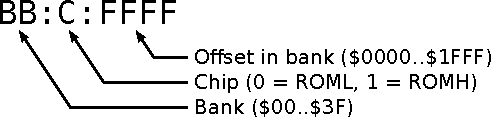
\includegraphics[scale=0.75]{src/address-scheme.pdf}
    \caption{Address scheme}
    \label{fig:address-scheme}
\end{figure}

\section{Scan the Keyboard}

When a cartridge is plugged into the C64, often the user has no other way to get to the BASIC prompt than unplugging the cartridge. EasyFlash has a switch or a jumper to avoid booting.

To make it easier for the user, scan the keyboard as early as possible in your start-up code. If one of the keys \raisebox{-2pt}{
\includegraphics[scale=0.4]{src/key-runstop.pdf}}, \raisebox{-2pt}{
\includegraphics[scale=0.4]{src/key-commodore.pdf}} or \raisebox{-2pt}{
\includegraphics[scale=0.4]{src/key-q.pdf}} is being held down, make the cartridge invisible and call the Kernal's reset vector. Remember that you can hide (“kill”) the cartridge by writing \$04 to \$DE02.

\section{LED Usage}

If there are no reasons to do it in a different way, you should use the LED like follows:

\begin{itemize}
  \item When the EasyFlash is active, the LED should be on
  \item When it is inactive (invisible mode), the LED should be off
  \item While the flash is being written, the LED should blink, e.g. toggle once per 256 bytes.
\end{itemize}
EAPI will take care for the last point. But you need to switch the LED on again after you finished the programming.

\section{Game States and High Scores}

Cartridges may save application specific data like game states and high scores to flash memory using EasyAPI. This is described in chapter \ref{easyapi}. Cartridge images (CRT files) should contain empty initialized data in this memory area. Do not rely on the assumption that EasyProg will erase the whole cartridge when a CRT file is flashed. Actually it will only erase sectors which are contained in the CRT file.

\section{Unused Data Areas}

Data areas which are contained in a cartridge image (CRT file) but not actually in use (i.e. padding areas and gaps) should be filled with \$ff. This may reduce the programming time.

\chapter{The EasyFlash Cartridge Format}\label{native-easyflash-cartridges}

Native EasyFlash Cartridges can use the full flash memory of 1 MiB. They can
use any kind of banking which is supported by the EasyFlash hardware in any way
they want. This is most probably the cartridge format you want to develop for.

EasySDK comes with some tools and code snippets to create, write and read
EasyFlash cartridges.

There are also other cartridge formats supported by the EasyFlash cartridge.
A short overview about these formats can be found in EasyFlash-EasyFS.pdf.

\section{Cartridge Boot Process}

As already mentioned, EasyFlash cartridges always start in Ultimax mode.
Therefore there is a small boot code required at the end of the ROMH flash chip
on bank 0 (00:1:1xxx). This start-up code is executed directly after a CPU reset.
The start-up code has to:

\begin{itemize}
  \item Provide the reset vector
  \item Initialize the CPU registers \$01 and \$00 (in this order)
  \item Initialize all I/O you need (SID, VIC-II etc.)
  \item Scan the keyboard
  \item Set up \$DE02 and start the stuff
\end{itemize}

A reference implementation for the start-up code can be found in
examples/banking-test.

If a native EasyFlash CRT wants to write to the flash memory, it may contain a
piece of code called EasyAPI. This is described in chapter \ref{easyapi}.

The memory area from 00:01:1800 to 00:01:1BFF is reserved for EasyAPI. So the
startup code and data can occupy e.g. the area 00:01:1C00 to 00:01:1FFF. A part
of this area may be used to embed a cartridge name, refer to chapter
\ref{cartridge-name} for more information.


\chapter{EasyAPI}\label{easyapi}

Applications can write to EasyFlash cartridges using a small library which
is called EasyAPI (EAPI). This application programming interface supports to
erase blocks of flash memory and write data to flash. Additionally it can be
used to read from flash memory. EasyAPI can be seen as a flash chip driver,
similar to drivers for your sound card or video card.

EAPI can be part of your cartridge software. If you put it at a special
position, EasyProg (the tool to write CRT images to cartridges) will
automatically update the EAPI code to the latest version when your cartridge is
written to flash memory. This is strongly recommended, because there are
different EasyFlash hardware versions which need an updated EAPI.

EasyAPI can also be used in programs running from disk. It can be loaded from a
file and used to write data to flash memory. Writing is done on a lower logical
level only, by directly addressing flash memory. There is no kind of flash file
system directly supported by EAPI.

\section{Using EasyAPI in Cartridges}

There is one very important feature of EAPI: When a CRT image which contains
the “EAPI” signature at the right place is written to a cartridge by EasyProg,
the EasyAPI memory area is replaced with the latest version of the EAPI code
for the actual flash chip type. The API of this code will remain compatible. To
add the EasyAPI code to your self-implemented CRT images, include the binary
(e.g. “eapi-am29f040-10”) at 00:01:1800 into your CRT image. Remember to
reserve 768 (\$0300) bytes of memory for future versions of EAPI.

Always embed the current version of EAPI for Am29F040 into your CRT, otherwise
it may not run on emulators because they usually emulate this chip.

\section{Using EasyAPI in Ordinary Programs}

EasyAPI can also be used in ordinary programs which are started e.g. from a
disk. They must search for a file called “eapi-????????-??” (note the number of
wildcards '?') on the current drive and load it to RAM. Programmers should not
link EasyAPI directly into their programs, otherwise it cannot be replaced by
newer versions of the file later.

\section{EasyAPI Memory Usage}

The functions of EasyAPI do not pollute the C64 RAM. All data they need is
stored in the a part of the EasyFlash RAM from \$DF80 to \$DFFF. One special
function named EAPIInit must be called first to initialize the jump table.
EAPIInit temporarily uses the zeropage locations \$4b and \$4c, but it backs
them up and restores them before the function returns.
When you use the RAM at \$df80 to \$dfff for something else, remember to call
EAPIInit again before using other EasyAPI functions.

\section{EasyAPI Code Position}

Before you call EAPIInit, you must load EAPI to any RAM area in the range
\$0200..\$7FFF or \$C000..\$CFFF. The first byte must be page aligned, EasyAPI
may be up to 768 (\$0300) bytes of size.

If you use EasyAPI from a cartridge, you must copy it from ROM to any RAM area
as described above. The reason is that the code uses bank switching and would
bank itself out otherwise.

\section{EasyAPI Signature}

\begin{table}[!htbp]
    \centering
    \begin{tabularx}{\textwidth}{ ccX }
        \toprule
        Offset & Length & Comment \\
        \midrule
        0   &   4   &   EasyAPI signature, always \$65 \$61 \$70 \$69 ("EAPI") \\[3pt]
        \bottomrule
    \end{tabularx}
\end{table}

This signature is only used to show the existence of EasyAPI. If the tool
EasyProg finds this signature, it can replace this memory area 00:1:1800 to
00:1:1BFF with a newer version of EasyAPI.

\section{EasyAPI Version String}

\begin{table}[!htbp]
    \centering
    \begin{tabularx}{\textwidth}{ ccX }
        \toprule
        Offset & Length & Comment \\
        \midrule
        4   &   16  &   EasyAPI version string, 0-terminated PETSCII \\[3pt]
        \bottomrule
    \end{tabularx}
\end{table}

This string contains the version of EasyAPI. It is for informational purpose only.

\section{EAPIInit}

Read Manufacturer ID and Device ID from the flash chip(s) and check if this
chip is supported by this driver. Prepare our private RAM for the other
functions of the driver. When this function returns, EasyFlash will be
configured to bank in the ROM area at \$8000..\$bfff.

Remember that this function must be called before any other EAPI function.

This function must be called with JSR loadAddress + 20 where loadAddress is the
address in RAM where you copied EasyAPI to.
It uses SEI, it restores all Flags except C before it returns. Do not call it
with D-flag set. \$01 must enable ROM at \$8000..\$bfff.

\begin{verbatim}
parameters:
      -
return:
      C   set: Flash chip not supported by this driver
          clear: Flash chip supported by this driver
      If C is clear:
      A   Device ID
      X   Manufacturer ID
      Y   Number of physical banks (>= 64) or
          number of slots (< 64) with 64 banks each
      If C is set:
      A   Error reason
changes:
      all registers are changed
\end{verbatim}

\section{EAPIWriteFlash - \$df80}

Write a byte to the given address. The address must be as seen in Ultimax
mode, i.e. do not use the base addresses \$8000 or \$a000 but \$8000 or \$e000.

When writing to flash memory only bits containing a '1' can be changed to
contain a '0'. Trying to change memory bits from '0' to '1' will result in
an error. You must erase a memory block to get '1' bits.

This function uses SEI, it restores all flags except C before it returns.
Do not call it with D-flag set. \$01 must enable the affected ROM area.

\begin{verbatim}
parameters:
      A   value
      XY  address (X = low), $8xxx/$9xxx or $Exxx/$Fxxx
return:
      C   set: Error
          clear: Okay
changes:
      Z,N <- value
\end{verbatim}


\section{EAPIEraseSector - \$df83}

Erase the sector at the given address. The bank number currently set and the
address together must point to the first byte of a 64 KiByte sector.

When erasing a sector, all bits of the 64 KiB area will be set to '1'.
This means that 8 banks with 8 KiB each will be erased, all of them either
in the LOROM chip when \$8000 is used or in the HIROM chip when \$e000 is
used.

This function uses SEI, it restores all flags except C before it returns.
Do not call it with D-flag set. \$01 must enable the affected ROM area.

\begin{verbatim}
parameters:
      A   bank
      Y   base address (high byte), $80 for LOROM, $a0 or $e0 for HIROM
return:
      C   set: Error
          clear: Okay
change:
      Z,N <- bank
\end{verbatim}


\section{EAPISetBank - \$df86}

Set the bank. This will take effect immediately for cartridge read access
and will be used for the next flash write or read command.

\begin{verbatim}
parameters:
      A   bank
return:
      -
changes:
      -
\end{verbatim}


\section{EAPIGetBank - \$df89}

Get the selected bank which has been set with EAPISetBank.
Note that the current bank number can not be read back using the hardware
register \$de00 directly, this function uses a mirror of that register in RAM.

\begin{verbatim}
parameters:
      -
return:
      A  bank
changes:
      Z,N <- bank
\end{verbatim}


\section{EAPISetPtr - \$df8c}

Set the pointer for EAPIReadFlashInc/EAPIWriteFlashInc.

\begin{verbatim}
parameters:
      A   bank mode, where to continue at the end of a bank
          $D0: 00:0:1FFF=>00:1:0000, 00:1:1FFF=>01:0:1FFF (lhlh...)
          $B0: 00:0:1FFF=>01:0:0000 (llll...)
          $D4: 00:1:1FFF=>01:1:0000 (hhhh...)
      XY  address (X = low) address must be in range $8000-$bfff
return:
      -
changes:
      -
\end{verbatim}


\section{EAPISetLen - \$df8f}

Set the number of bytes to be read with EAPIReadFlashInc.

\begin{verbatim}
parameters:
      XYA length, 24 bits (X = low, Y = med, A = high)
return:
      -
changes:
      -
\end{verbatim}


\section{EAPIReadFlashInc - \$df92}

Read a byte from the current pointer from EasyFlash flash memory.
Increment the pointer according to the current bank wrap strategy.
Pointer and wrap strategy have been set by a call to EAPISetPtr.

The number of bytes to be read may be set by calling EAPISetLen.
EOF will be set if the length is zero, otherwise it will be decremented.
Even when EOF is delivered a new byte has been read and the pointer
incremented. This means the use of EAPISetLen is optional.

\begin{verbatim}
parameters:
      -
return:
      A   value
      C   set if EOF
changes:
      Z,N <- value
\end{verbatim}


\section{EAPIWriteFlashInc - \$df95}

Write a byte to the current pointer to EasyFlash flash memory.
Increment the pointer according to the current bank wrap strategy.
Pointer and wrap strategy have been set by a call to EAPISetPtr.
In case of an error the position is not inc'ed.

\begin{verbatim}
parameters:
      A   value
return:
      C   set: Error
          clear: Okay
changes:
      Z,N <- value
\end{verbatim}


\section{EAPISetSlot - \$df98}

Set the slot. This function is only available if EAPIInit reported
multiple slots.

Software which does not need to change the slot number should not need to
use this function. So usually only EasyProg or similar programs need to call
this.

This will take effect immediately for cartridge read access
and will be used for the next flash write or read command.

\begin{verbatim}
parameters:
      A   slot
return:
      -
changes:
      -
\end{verbatim}

\chapter{Cartridge Name}\label{cartridge-name}

New EasyFlash implementations show EasyFlash CRTs in a menu. CRT files may
contain a default name for a menu entry at a special place directly behind the
memory area which is reserved for EAPI, as shown in table \ref{tab:cartridge-name}.

\begin{table}[!htbp]
    \centering
    \begin{tabularx}{\textwidth}{ cX }
        \toprule
        Position & Content \\
        \midrule
        00:1:1800 & EAPI \\[3pt]
        00:1:1b00 & Magic "EF-Name:", PETSCII (65 66 2d 6e 41 4d 45 3a) \\[3pt]
        00:1:1b08 & Name in upper/lower case PETSCII, up to 16 characters, no gfx symbols, padded to 16 bytes with binary 0. \\[3pt]
        00:1:1b18 & Start-up code or other data \\[3pt]
        \bottomrule
    \end{tabularx}
    \caption{EasyFlash Cartidge Name}
    \label{tab:cartridge-name}
\end{table}

Example:

\footnotesize
\begin{verbatim}
i fb00
>C:fb00 EF-Name:Myth@@@@@@@@@@@@................

m fb00
>C:fb00  65 66 2d 6e  41 4d 45 3a  6d 59 54 48  00 00 00 00   ef-nAME:mYTH....
>C:fb10  00 00 00 00  00 00 00 00  ff ff ff ff  ff ff ff ff   ................
\end{verbatim}
\normalsize

\end{document}

